\section{Experiments}\label{sec:experiment}

To prove the effectiveness of \ours, we conduct comprehensive experiments and present the setup, main results, and analysis in this section. Specifically, we focus on the following research questions (RQ): \textbf{RQ1:}
Does \ours \space outperform other directly comparable methods? \textbf{RQ2:} Does the main components of \ours \space work effectively? \textbf{RQ3:} How does \ours \space progressively enhance the agent's reasoning capability for the KBQA task with outcome-only supervision? \textbf{RQ4:} Does \ours \space generates flexible and robust reasoning trajectories?


\subsection{Experiment Setup}
\textbf{Dataset and Metrics}. We evaluate \ours \space on three widely-used KBQA datasets: WebQSP, CWQ, and the generalization-focused GrailQA, using a subset of the official testing data. Following existing work~\citep{xiong2024interactive}, we primarily evaluate the F1 metrics, supplemented by Random Hits@1(RHits@1) and EM score. As our approach does not rely on semantic parsing, we do not report logical form accuracy~\citep{gu2021beyond}. 

\textbf{Baselines}. We compare \ours \space against two main categories of methods: prompting-based and fine-tuning-based methods. For the former, we include a diverse range of prompting strategies, from direct prompting, such as IO, CoT, etc., and agent-based reasoning method Interactive-KBQA~\citep{xiong2024interactive}. To ensure a fair comparison and reproducibility, we report the scores for these methods directly from their original publications. For the fine-tuning-based methods, we select SOTA methods finetuned on full data, include RnG-KBQA~\citep{ye2022rng} and TIARA~\citep{shu2022tiara}, and the directly comparable low-source methods, which are finetuned on low-source data, includes agentic approaches like SFT-traj.~\citep{xiong2024interactive}, KBQA-o1~\citep{luokbqao1}, and MCTS-KBQA~\citep{xiong2025mcts}.

Further details on the datasets, baselines, evaluation protocol, and implementation are provided in Appendix~\ref{app:setup}.



\begin{table*}[!t]
  \centering
  \caption{Experiment Results (in percentage) on WebQSP, CWQ, and GrailQA. The \textbf{Bold} and \underline{underlined} numbers indicate the best and second-best low-resource performance.}
  \label{tab:all-three}
  \resizebox{\linewidth}{!}{%
  \begin{tabular}{c c c c c c c c c c}
    \toprule
    \multirow{2}{*}{Method} & \multirow{2}{*}{Backbone} &
      \multicolumn{2}{c}{WebQSP} & \multicolumn{2}{c}{CWQ} & \multicolumn{4}{c}{GrailQA} \\
    \cmidrule(lr){3-4}\cmidrule(lr){5-6}\cmidrule(lr){7-10}
     & & Overall~F1 & RHits@1 & Overall~F1 & EM & I.I.D. & Compositional & Zero-shot & Overall \\
    \midrule
    \multicolumn{10}{c}{\textit{Prompting Methods}} \\
    \midrule
    IO        & GPT-4-turbo     & 39.3 & 45.5 & 33.9 & 45.7 & --- & --- & --- & 29.4 \\
    CoT       & GPT-4-turbo     & 39.7 & 47.5 & 33.7 & 43.7 & --- & --- & --- & 28.1 \\
    CoT+SC    & GPT-4-turbo     & 39.0 & 47.1 & 36.6 & 47.5 & --- & --- & --- & 29.6 \\
    KB-BINDER & Codex-davinci-002 & 52.6 & --- & --- & --- & 43.3 & 36.6 & 44.0 & 42.2 \\
    KB-Coder  & GPT-3.5-turbo     & 55.7 & --- & --- & --- & 45.5 & 38.6 & 47.3 & 44.9 \\
    ARG-KBQA  & GPT-3.5-turbo     & 58.8 & --- & --- & --- & 51.5 & 41.8 & 52.1 & 48.5 \\
    % \multicolumn{10}{c}{\textit{Prompting-based Agentic Methods}} \\
    Interactive-KBQA & GPT-4-turbo     & 71.2 & 72.5 & 49.1 & 59.2 & --- & --- & --- & --- \\
    \midrule
    \multicolumn{10}{c}{\textit{Fine-tune-based Methods}} \\
    \midrule
    RnG-KBQA & BERT-base-uncased         & 75.6 & ---   & ---   & ---   & 89.0 & 68.9 & 74.7 & 76.9 \\
    TIARA    & BERT-base-uncased         & 78.9 & 75.2 & ---   & ---   & 91.2 & 74.8 & 80.7 & 81.9 \\
    \midrule
    SFT-traj. & Llama2-7B     & 57.5 & 59.9 & 42.2 & 48.8 & 54.2 & 45.8 & 44.2 & 48.5 \\
    MCTS-KBQA         & Llama-3.1-8B & \underline{76.0} & 76.2 & \underline{66.8} & \underline{75.2} & --- & --- & --- & --- \\
    KBQA-o1           & Qwen2.5-7B   & 57.8 & ---   & ---   & ---   & \textbf{84.4} & \textbf{77.0} & \underline{75.7} & \underline{77.9} \\
    \midrule
    % \multicolumn{10}{c}{\textit{SFT-based Agentic Methods}} \\
    \ours-cold start & Qwen2.5-Coder-7B & 56.1 & 66.3 & 54.8 & 59.8 & 60.6 & 63.5 & 67.2 & 63.1 \\
    \rowcolor{blue!8}
    \ours         & Qwen2.5-Coder-7B & \textbf{77.2} & \textbf{80.1} & \textbf{68.3} & \textbf{75.7} & \underline{81.1} & \underline{70.6} & \textbf{84.1} & \textbf{80.5} \\
    \bottomrule
  \end{tabular}}
\end{table*}


\begin{table}[h]
  \centering
  \small
  \caption{Training instances (Train) and evaluation result with consumption (Evaluation), where 'Time' represents the average number of rollouts required per question at inference, normalized to our method (1x).}
  \label{tab:sample_used}
  \resizebox{\linewidth}{!}{%
  \begin{tabular}{l c c c c c c c c c c}
    \toprule
    \multirow{3}{*}{Model}
      & \multicolumn{4}{c}{Train}
      & \multicolumn{6}{c}{Evaluation} \\
    \cmidrule(lr){2-5}\cmidrule(lr){6-11}
      & \makecell{P.S.\\\#Inst.}
      & \multicolumn{3}{c}{\makecell{O.S.\#Inst.}}
      & \multicolumn{2}{c}{CWQ}
      & \multicolumn{2}{c}{WebQSP}
      & \multicolumn{2}{c}{GrailQA} \\
    \cmidrule(lr){3-5}\cmidrule(lr){6-7}\cmidrule(lr){8-9}\cmidrule(lr){10-11}
      &  & WebQSP & CWQ & GrailQA
      & Time & F1 & Time & F1 & Time & F1 \\
    \midrule
    MCTS\text{-}KBQA
      & 750 & 2743 & \textbf{2843} & \textemdash
      & \(3.24\times\) & 66.8 & \(2.91\times\) & 76.0 & \textemdash & \textemdash \\
    KBQA\text{-}o1
      & 240 & 2929 & \textemdash & 43851
      & \textemdash & \textemdash & \(6\times\) & 57.8 & \(6\times\) & 77.9 \\
    \textbf{Ours}
      & \textbf{0} & \textbf{2414} & \underline{4699} & \textbf{3563}
      & \(1\times\) & \textbf{68.3} & \(1\times\) & \textbf{77.2} & \(1\times\) & \textbf{80.5} \\
    \bottomrule
  \end{tabular}%
  }
\end{table}
\subsection{Main Results - RQ1}
To evaluate the performance of \ours, we conducted comprehensive experiments on three datasets, with the results presented in Table~\ref{tab:all-three}. For additional context on the efficiency of our method, we compare the number of samples used during training with the number of rollouts used during inference in Table~\ref{tab:sample_used}. Taken together, these results demonstrate that \ours establishes a new state-of-the-art for low-resource KBQA across all benchmarks. This shows the effectiveness of our approach, which can be analyzed from three key aspects.

First, \ours \space significantly outperforms all directly comparable low-resource baselines, particularly on the more complex CWQ and the generalization-focused GrailQA datasets. Meanwhile, it nearly closes the gap with fully-supervised methods while using only a fraction of the data (~10k outcome-supervised samples vs. ~60k fully-annotated queries), highlighting its exceptional data efficiency. 


Second, results prove that the outcome-supervised multi-stage training strategy is effective than the process-supervised SFT strategy.
Results in the last two blocks of Table~\ref{tab:all-three} indicate that \ours \space our approach consistently outperforms leading process-supervised SFT baselines. On GrailQA, \ours \space achieves an F1 score of 80.5\%, which represents a 3.3\% relative improvement over the prior state-of-the-art method KBQA-o1 while using 12× less training data (3.5k vs. 43.8k samples). While performance is slightly lower on GrailQA's I.I.D. and compositional subsets, which favor extensive training data to cover specific patterns, our method demonstrates a relative improvement of up to 11.1\% on the zero-shot subset. This proves its superior ability to reason effectively on truly unseen questions.

Furthermore, beyond higher overall scores, \ours \space is more efficient in both supervision and inference. In terms of supervision, as detailed in the ``Train'' columns of Table~\ref{tab:sample_used}, \ours \space uses zero process-supervised (P.S.) instances and a comparable or smaller number of outcome-supervised (O.S.) samples than MCTS-based competitors. As montioned before, \ours \space outperforms KBQA-o1 on GrailQA while using much fewer supervised samples. In terms of inference, as shown in the ``Evaluation'' columns of Table~\ref{tab:sample_used}, \ours \space employs a single linear reasoning pass and avoids the costly sampling required by MCTS, reducing latency by 3.2–6 times.
These results support outcome supervision as a more effective and efficient alternative to incremental SFT on pre-defined or explored paths. 

Finally, \ours \space unlocks SOTA reasoning capabilities in smaller models. As shown in the first block of Table~\ref{tab:all-three}, \ours \space consistently outperforms prompting-based methods that rely on significantly larger models like GPT-4-turbo by at least 6\% at F1. This demonstrates an essential improvement in the model's intrinsic reasoning ability.

\begin{table*}[!t]
  \centering
  \caption{Ablation Study on Three KBQA Datasets.}
  \label{tab:ablation}
  \resizebox{\textwidth}{!}{ %
  \begin{tabular}{lcccccccc}
    \toprule
    \multirow{2}{*}{\textbf{Model}} &
      \multicolumn{4}{c}{\textbf{GrailQA}} &
      \multicolumn{2}{c}{\textbf{WebQSP}} &
      \multicolumn{2}{c}{\textbf{CWQ}} \\
    \cmidrule(lr){2-5} \cmidrule(lr){6-7} \cmidrule(l){8-9}
    & IID & Comp. & Zero-shot & Overall F1
    & F1 & Hits@1
    & F1 & EM \\
    \midrule
    \ours              & \textbf{81.1} & 70.6 & \textbf{84.1} & \textbf{80.5} & \textbf{77.2} & 80.1 & \textbf{68.3} & \textbf{75.7} \\
    \midrule
    \multicolumn{9}{l}{w/o reward curriculum} \\
    \quad EM as Reward      & 45.5 & 50.6 & 73.6 & 62.8 & 73.8 & 76.1 & 50.2 & 55.0 \\
    \quad F1 as Reward             & 68.7 & \textbf{77.6} & 78.6 & 76.0 & 71.9 & 77.0 & 58.3 & 59.8 \\
    \quad F0.5 as Reward           & 79.1 & 68.2 & 82.6 & 78.7 & 76.3 & \textbf{80.9} & 67.2 & 74.7 \\
    \quad F1+F0.5 as Reward  & 74.9 & 65.5 & 82.6 & 76.1 & 73.8 & 77.0 & 64.6 & 66.1 \\
    \midrule
    \addlinespace[1pt]
    w/o RL (cold-start)        & 60.6 & 63.5 & 67.2 & 63.1 & 56.7 & 64.9 & 50.5 & 59.8 \\
    w/o upsampling             & 52.5 & 53.0 & 62.3 & 60.2 & 56.1 & 66.3 & 54.8 & 52.7 \\
    \bottomrule
  \end{tabular}
  }
\end{table*}
\subsection{Ablation Study - RQ2}
To verify the effectiveness of our key designs, we conduct a comprehensive ablation study, and the results are presented in Table~\ref{tab:ablation}. First, we assess the reward curriculum by replacing our proposed easy-to-hard ($F_{0.5}$-then-$F_{1}$) strategy, give the result using EM, $F_1$, $F_{0.5}$, and revered strategy $F_1$-then-$F_{0.5}$ as reward, respectively. Next, we evaluate the contribution of the entire RL stage by removing it altogether. Finally, we remove the data sampling strategy from the initial cold-start phase. The results confirm that each component is integral to the model's performance, as removing or modifying any of them leads to a noticeable degradation.

\textbf{Effectiveness of the Easy-to-Hard Reward Curriculum.}
The first block of Table~\ref{tab:ablation} shows the effectiveness of the Easy-to-Hard Reward Curriculum. Take the GrailQA dataset as an example, we observe that an overly simplistic signal like EM is insufficient for exploration; it induces "over-recall reward hacking," resulting in a massive drop in the $F_1$ score on GrailQA. Meanwhile, a stricter F1 reward is too punishing early on, leading to a -4.5\% F1 drop. Notably, reversing the curriculum to a hard-to-easy schedule ($F_1$-then-$F_{0.5}$) also degrades performance (-4.4\% F1 drop). This confirms our hypothesis: starting with an ``easy task'' encourages broad exploration to discover correct reasoning paths, while the subsequent ``hard task'' refines the agent's ability to achieve a better balance between precision and recall.

\textbf{Critical Contribution of the RL Stage.} From the second block of Table~\ref{tab:ablation}, we can observe that removing the entire RL-stage causes at least 17.4\% absolute drop in the F1 score. This large gap suggests that RL-based exploration is essential for refining the agent's reasoning capability beyond initial supervised learning.

\textbf{Importance of Upsampling in the Cold-Start Stage.}
Finally, as the last row shows, removing the up-sampling of infrequent question types leads to poor performance on those specific categories. This underscores the importance of our sampling strategy for building a model that can generalize across a diverse range of reasoning patterns.

\subsection{Analysis - RQ3}

To answer the RQ3 and investigate how \ours \space progressively enhances the agent's reasoning capability under the outcome-only supervision, we analyze from the train dynamics, the evolution of its reasoning robustness and diversity, and the comparative performance against process-supervised methods. 

\subsubsection{Analysis of Training Dynamics with Outcome-Only Supervision}
\label{sec:trian_dym}
As shown in Fig.~\ref{fig:train_dynamic}, to track the evolution of the model's capabilities during training, we present the curves of (a) training reward, (b) response length (token), (c) turns of interaction, and (d) the number of invalid tool calls along the training step. It can be seen that the agent's strategy clearly transitions from \textbf{broad exploration} to \textbf{efficient exploitation}: initially, the agent explores inefficiently, which is reflected in high response lengths and turn counts for a low reward. As training progresses, these trends reverse: the reward consistently rises while the metrics for response length, turns, and invalid tool calls all significantly decrease. This dynamic illustrates a fundamental improvement in the agent's complex question-solving process, not just a superficial optimization of rewards.

\subsubsection{Analysis of Reasoning Capability}

\begin{figure*}
    \centering
    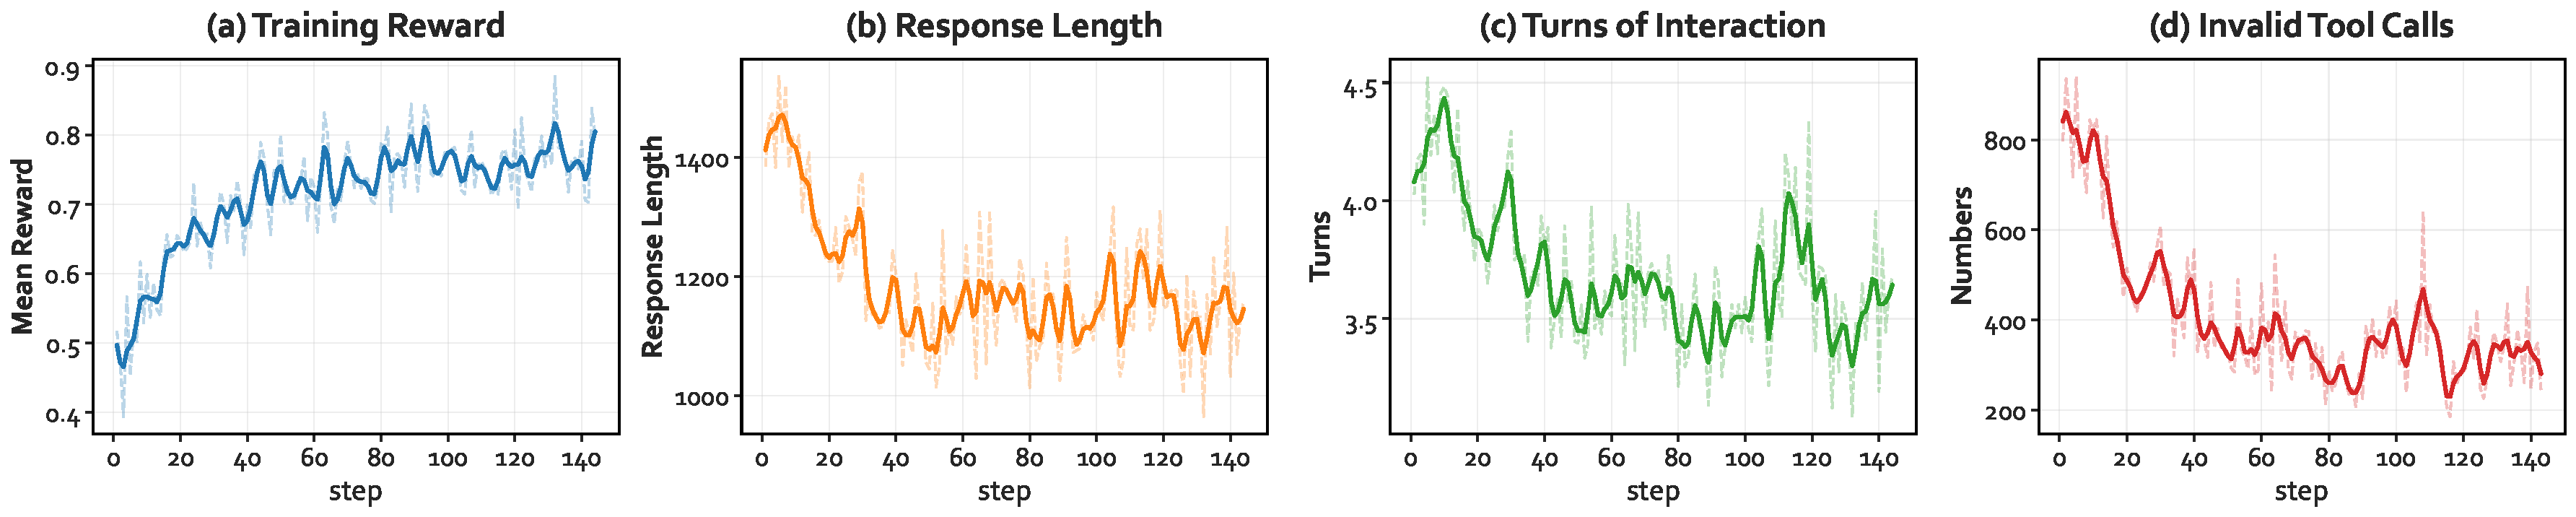
\includegraphics[width=1\textwidth]{figures/fixed_metrics_plot.pdf}
    \caption{Training curves for \ours, illustrating: (a) training reward, (b) response length, (c) interaction turns, and (d) the number of invalid tool calls.}
    \label{fig:train_dynamic}
\end{figure*}
\begin{figure}
    \centering
    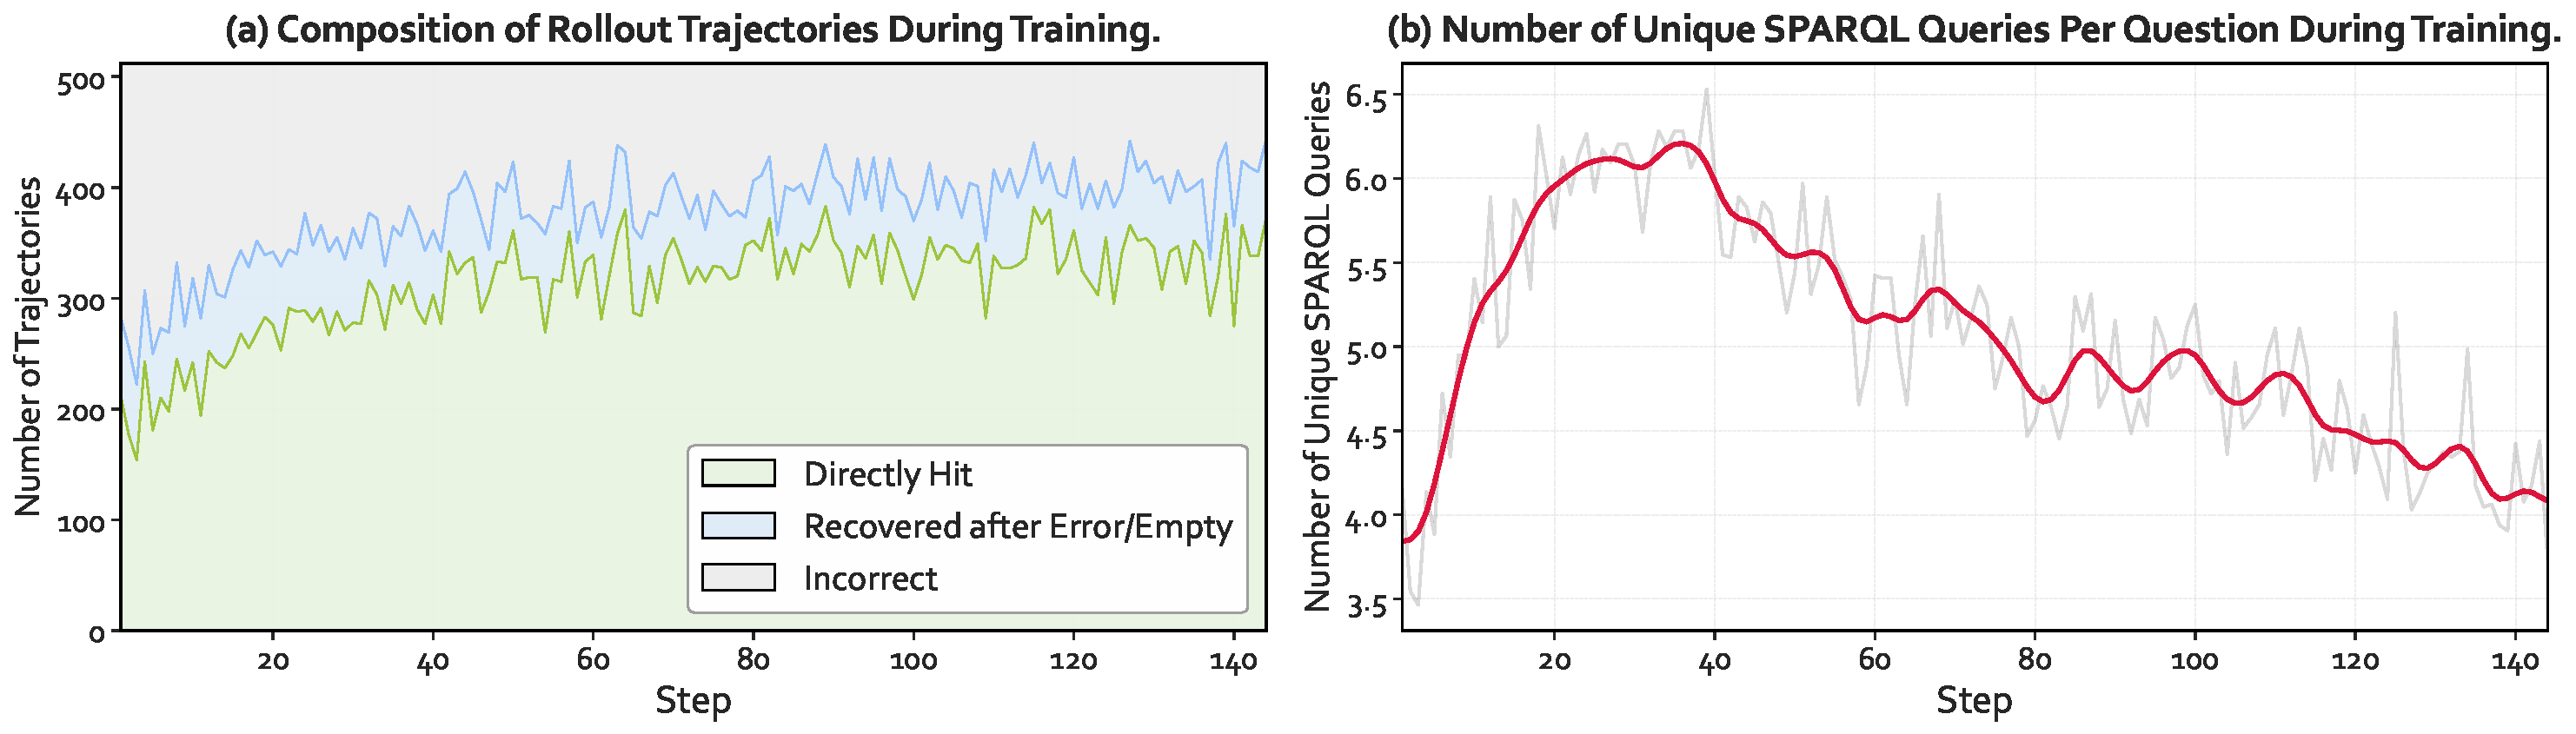
\includegraphics[width=1\linewidth]{figures/combined_charts.pdf}
    \caption{Evolution of Robustness and Flexibility during training: (a) Robustness, shown by the composition of rollout trajectories, and (b) Flexibility, shown by the number of unique SPARQL queries per question.}
    \label{fig:flex_and_rob}
\end{figure}
To provide a deeper analysis of whether the model's reasoning ability is enhanced, particularly concerning the robustness and flexibility lacking in SFT methods, we examine the evolution of the agent's reasoning behavior. Fig.~\ref{fig:flex_and_rob}(a) illustrates its robustness by showing the composition of rollout trajectories, categorized as: "Directly Hit," for trajectories where the final prediction hits at least one gold answers; "Recovered after Error/Empty," for those that hit at least one gold answers after encountering an intermediate error or empty observation; and "Incorrect," for trajectories where the final prediction fails to find any gold answerss. The figure shows that the proportion of successful trajectories ("Directly Hit" and "Recovered") steadily increases during training, This confirms that the agent learns to effectively recover from imperfect feedback, a direct advantage of our outcome supervision approach. In contrast, process supervision encourages the model to simply replicate pre-defined trajectories from the training data, and thus fails to incentivize this type of recovery behavior.

Fig.~\ref{fig:flex_and_rob}(b) measures flexibility by plotting the diversity of trajectories, which we define as the number of unique final SPARQL queries generated for the same question across the rollouts. It can be seen that the agent initially broadens its search for a wide range of solutions before consolidating on a compact set of the most reliable ones, which is consistent with the process discussed in Sec.~\ref{sec:trian_dym}. This indicates that outcome-only supervision naturally fosters an exploration-then-convergence behavior, where the agent ultimately retains sufficient solution diversity to effectively address the lack of flexibility inherent in process-supervised methods.

\subsubsection{Analysis of Process Reward}
To explore whether incorporating process supervision in addition to outcome-only supervision benefits model performance, we experimented by incorporating necessary process-level penalties for behaviors including hallucinations and timeouts. Specifically, we define a hallucination as a tool call containing a relation or type that is not present in the observation history, while a timeout query denotes a call that results in a 300 second timeout. We applied a negative reward of -0.2 for each occurrence of these behaviors, with the total accumulated penalty capped at -0.5. We then compared our full model against two variants incorporating these Process Rewards (P.R.): one applying the penalties throughout the entire RL training (P.R.@RL-phase-1\&2), and another applying them only during the second stage (P.R.@RL-phase-2).
The results clearly demonstrate that introducing penalties for any intermediate behaviors, even for intuitively negative ones, degrades final performance. We hypothesize  that in KBQA tasks, where the correctness of answers can be explicitly verified, process-level rewards may interfere with the agent’s capacity to form a robust trial-and-error exploration strategy, as they tend to prematurely penalize exploratory trajectories that could eventually achieve correct results.
\begin{table}[htbp]
\centering
\caption{Performance comparison of different models and training stages on the WebQSP, CWQ, and GrailQA.}
\label{tab:process}
\begin{tabular}{l cc cc cc}
\toprule
\multirow{2}{*}{\textbf{Model}} & \multicolumn{2}{c}{\textbf{WebQSP}} & \multicolumn{2}{c}{\textbf{CWQ}} & \multicolumn{2}{c}{\textbf{GrailQA}} \\
\cmidrule(r){2-3} \cmidrule(r){4-5} \cmidrule(l){6-7}
 & F1 & Hit@1 & F1 & EM & F1 & EM \\
\midrule
P.R.@RL-phase-1\&2  & 71.5 & 75.3 & 64.9 & 72.7 & 73.0 & 76.2 \\
P.R.@RL-phase-2 & 73.3 & 78.2 & 68.0 & 74.8 & 78.1 & 81.0 \\
\ours         & \textbf{77.2} & \textbf{80.1} & \textbf{68.3} & \textbf{75.7} & \textbf{80.5} & \textbf{83.7} \\
\bottomrule
\end{tabular}
\end{table}

\subsection{Case Study - RQ4}

To concretely demonstrate the advanced reasoning capabilities of \ours, we present a qualitative case study with two detailed examples in Appendix~\ref{app:case}. These examples highlight the agent's ability to: (1) robustly recover from erroneous feedback; (2) flexibly use tools to find correct answers via reasoning trajectories that differ from the gold SPARQL. These cases serve as strong evidence of the robustness and flexibility fostered by the proposed \ours\space approach.

In addition, we conduct error analysis, which is presented in Appendix~\ref{app:error}.










